\documentclass[11pt]{article}
\usepackage[textwidth=18.0cm, textheight=23.0cm, top=2.0cm]{geometry}
\usepackage{pst-all}
\usepackage{amssymb}
\usepackage{tikz}
\usepackage{underscore}\begin{document}
\pagestyle{empty}


ClassName: \underline{\textbf{Class_03.2bp-18}}
\par
BinSize: \underline{\textbf{40 × 40}}
\par
ReduceSize: \underline{\textbf{40 × 40}}
\par
TypeNum: \underline{\textbf{39}}
\par
Num: \underline{\textbf{40}}
\par
OutS: \underline{\textbf{11200}}
\par
InS: \underline{\textbf{10710}}
\par
Rate: \underline{\textbf{0.956}}
\par
UB: \underline{\textbf{7}}
\par
LB0: \underline{\textbf{7}}
\par
LB: \underline{\textbf{7}}
\par
LBWithCut: \underline{\textbf{7}}
\par
NodeCut: \underline{\textbf{0}}
\par
ExtendedNodeCnt: \underline{\textbf{1}}
\par
GenNodeCnt: \underline{\textbf{1}}
\par
PrimalNode: \underline{\textbf{2}}
\par
ColumnCount: \underline{\textbf{143}}
\par
TotalCutCount: \underline{\textbf{196}}
\par
RootCutCount: \underline{\textbf{196}}
\par
LPSolverCnt: \underline{\textbf{210}}
\par
PricingSolverCnt: \underline{\textbf{209}}
\par
BranchAndBoundNum: \underline{\textbf{1}}
\par
isOpt: \underline{\textbf{true}}
\par
TimeOnPrimal: \underline{\textbf{63.651 s}}
\par
TimeOnPricing: \underline{\textbf{328.824 s}}
\par
TimeOnRmp: \underline{\textbf{0.242 s}}
\par
TotalTime: \underline{\textbf{329.322 s}}
\par
\newpage


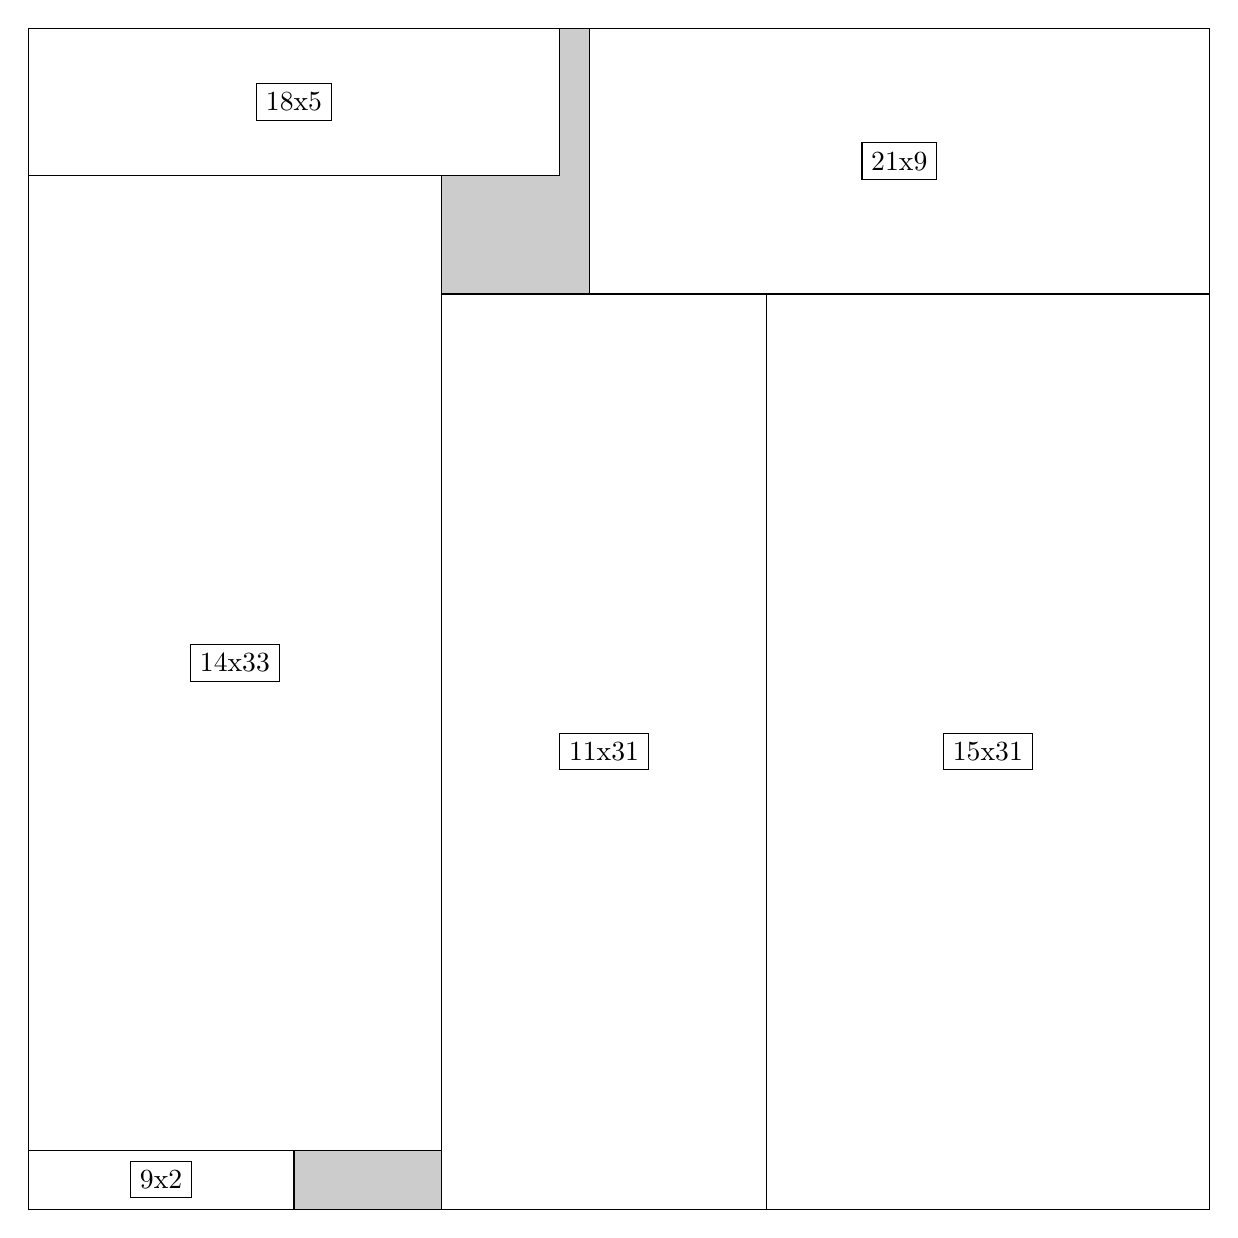
\begin{tikzpicture}[shorten >=1pt,scale=1.0,every node/.style={scale=1.0},->]
\tikzstyle{vertex}=[circle,fill=black!25,minimum size=14pt,inner sep=0pt]
\filldraw[fill=gray!40!white, draw=black] (0,0) rectangle (15.0,15.0);
\foreach \name/\x/\y/\w/\h in {14x33/0.0/0.75/5.25/12.375,18x5/0.0/13.125/6.75/1.875,9x2/0.0/0.0/3.375/0.75,11x31/5.25/0.0/4.125/11.625,21x9/7.125/11.625/7.875/3.375,15x31/9.375/0.0/5.625/11.625}
\filldraw[fill=white!40!white, draw=black] (\x,\y) rectangle node[draw] (\name) {\name} ++(\w,\h);
\end{tikzpicture}


w =14 , h =33 , x =0 , y =2 , v =462
\par
w =18 , h =5 , x =0 , y =35 , v =90
\par
w =9 , h =2 , x =0 , y =0 , v =18
\par
w =11 , h =31 , x =14 , y =0 , v =341
\par
w =21 , h =9 , x =19 , y =31 , v =189
\par
w =15 , h =31 , x =25 , y =0 , v =465
\par
\newpage


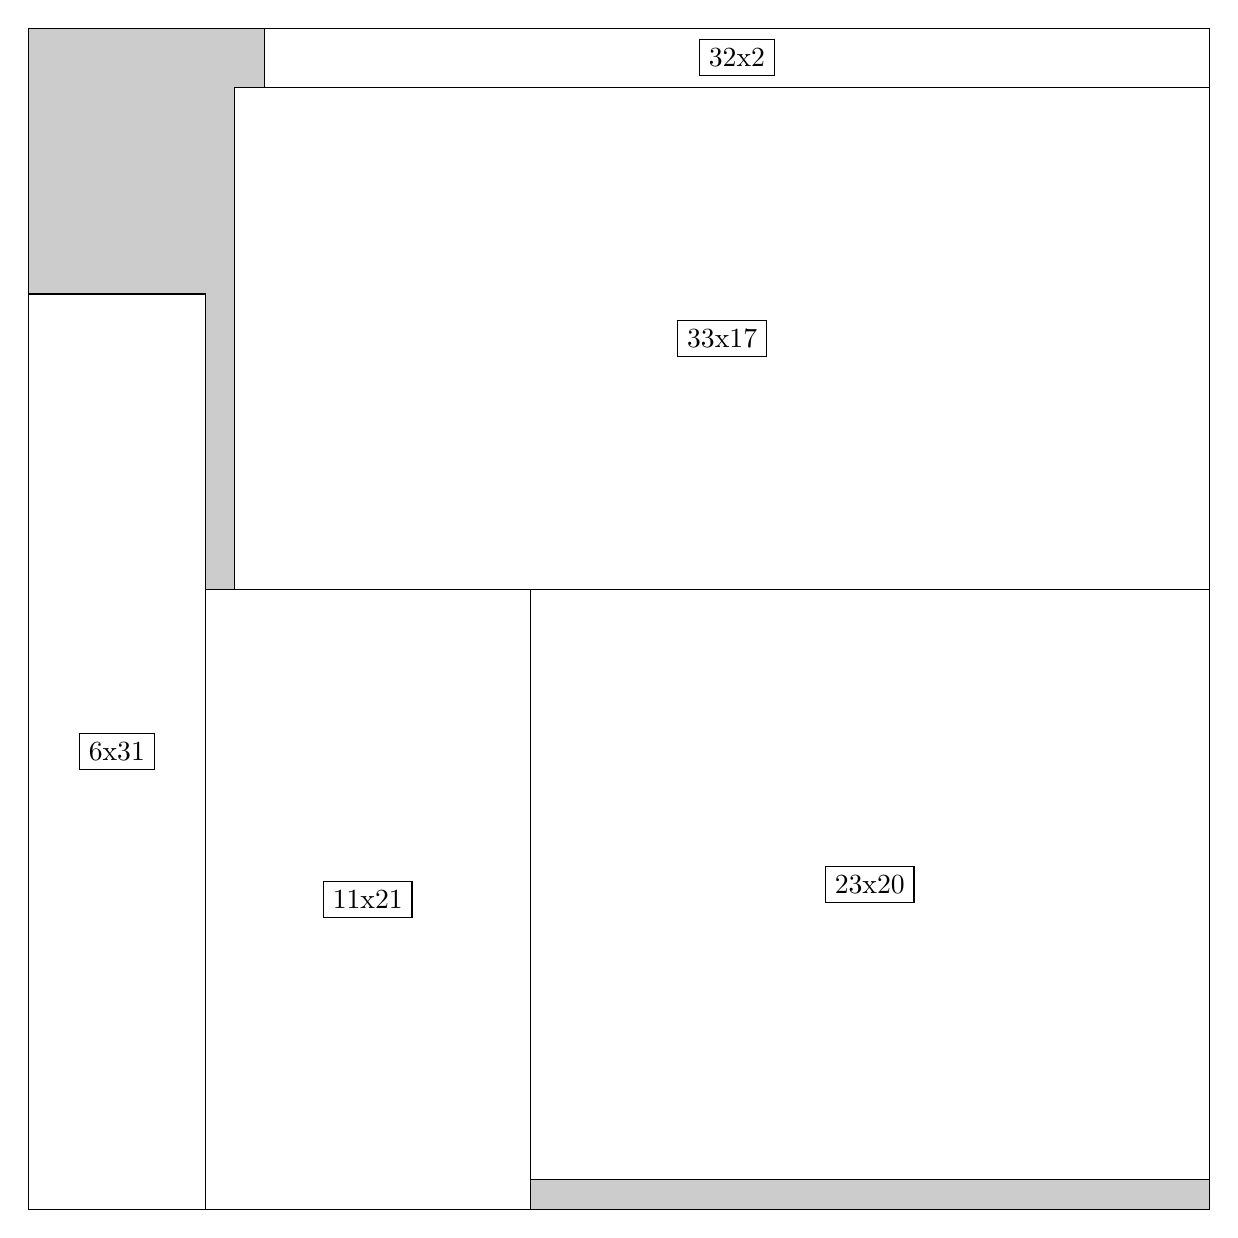
\begin{tikzpicture}[shorten >=1pt,scale=1.0,every node/.style={scale=1.0},->]
\tikzstyle{vertex}=[circle,fill=black!25,minimum size=14pt,inner sep=0pt]
\filldraw[fill=gray!40!white, draw=black] (0,0) rectangle (15.0,15.0);
\foreach \name/\x/\y/\w/\h in {6x31/0.0/0.0/2.25/11.625,11x21/2.25/0.0/4.125/7.875,33x17/2.625/7.875/12.375/6.375,32x2/3.0/14.25/12.0/0.75,23x20/6.375/0.375/8.625/7.5}
\filldraw[fill=white!40!white, draw=black] (\x,\y) rectangle node[draw] (\name) {\name} ++(\w,\h);
\end{tikzpicture}


w =6 , h =31 , x =0 , y =0 , v =186
\par
w =11 , h =21 , x =6 , y =0 , v =231
\par
w =33 , h =17 , x =7 , y =21 , v =561
\par
w =32 , h =2 , x =8 , y =38 , v =64
\par
w =23 , h =20 , x =17 , y =1 , v =460
\par
\newpage


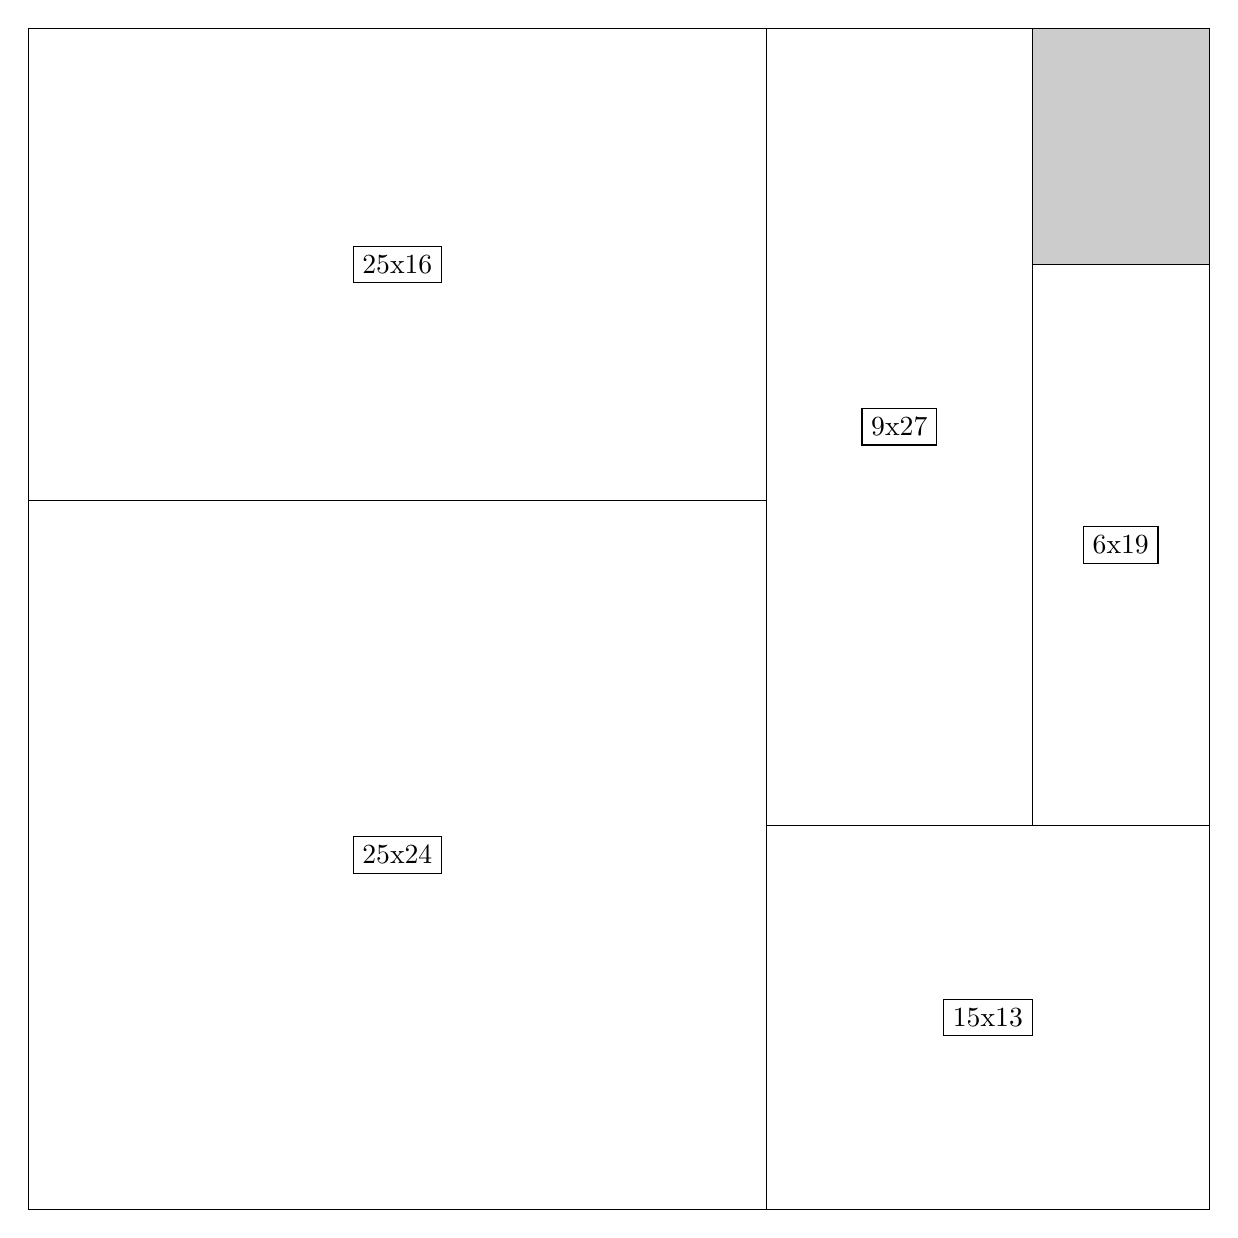
\begin{tikzpicture}[shorten >=1pt,scale=1.0,every node/.style={scale=1.0},->]
\tikzstyle{vertex}=[circle,fill=black!25,minimum size=14pt,inner sep=0pt]
\filldraw[fill=gray!40!white, draw=black] (0,0) rectangle (15.0,15.0);
\foreach \name/\x/\y/\w/\h in {25x24/0.0/0.0/9.375/9.0,25x16/0.0/9.0/9.375/6.0,9x27/9.375/4.875/3.375/10.125,15x13/9.375/0.0/5.625/4.875,6x19/12.75/4.875/2.25/7.125}
\filldraw[fill=white!40!white, draw=black] (\x,\y) rectangle node[draw] (\name) {\name} ++(\w,\h);
\end{tikzpicture}


w =25 , h =24 , x =0 , y =0 , v =600
\par
w =25 , h =16 , x =0 , y =24 , v =400
\par
w =9 , h =27 , x =25 , y =13 , v =243
\par
w =15 , h =13 , x =25 , y =0 , v =195
\par
w =6 , h =19 , x =34 , y =13 , v =114
\par
\newpage


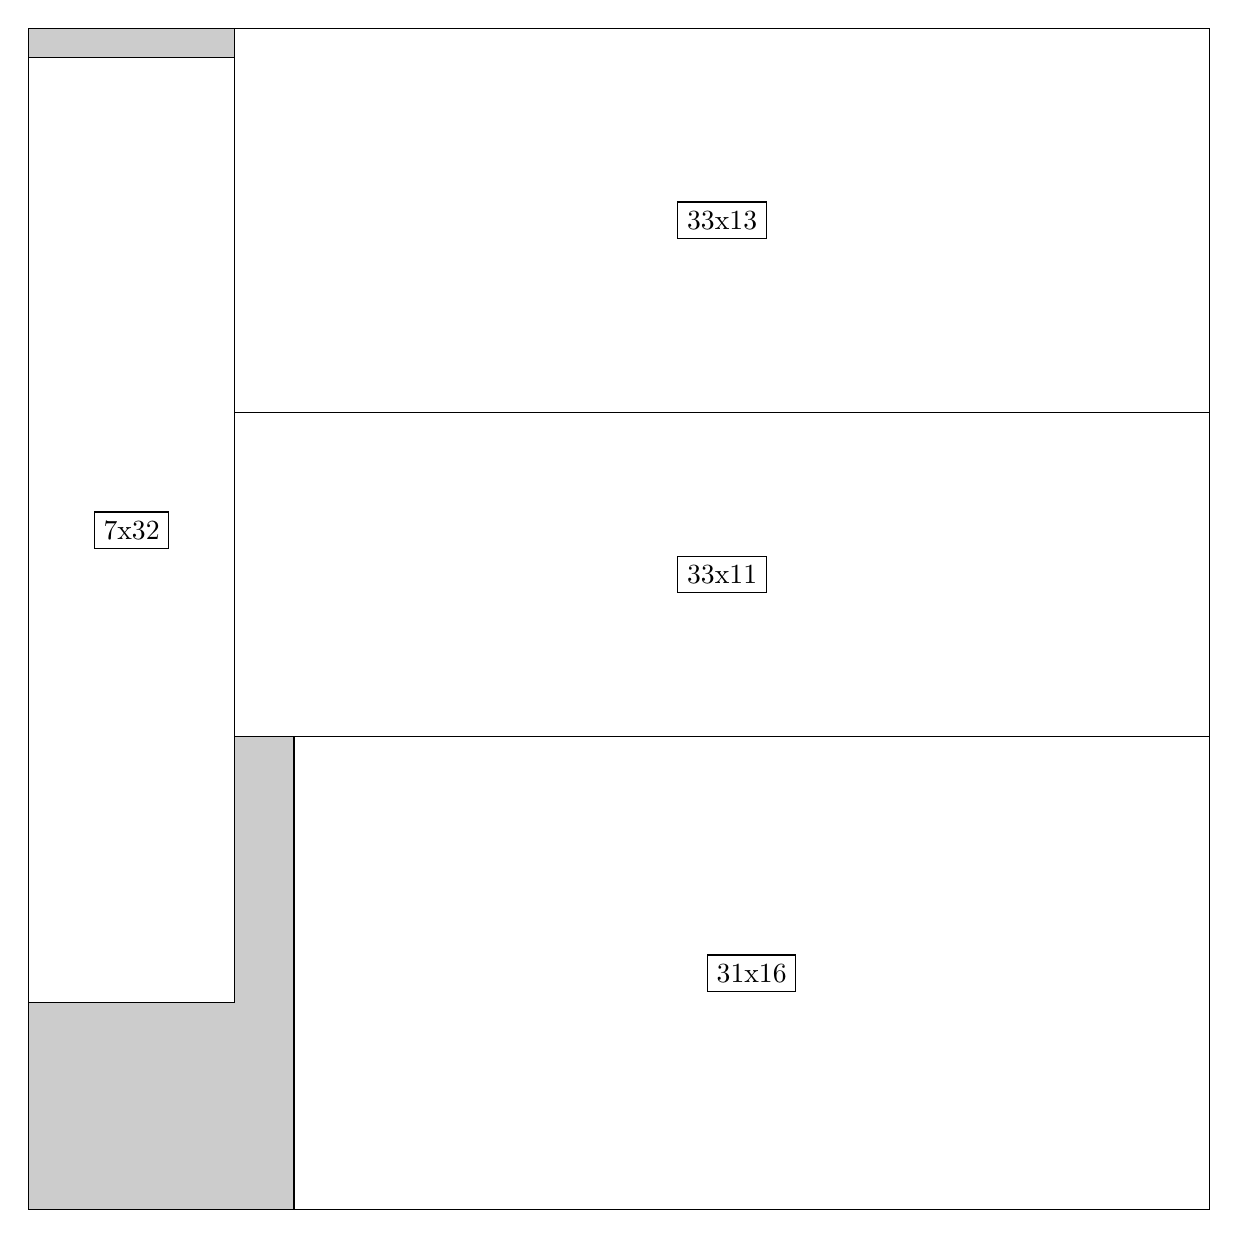
\begin{tikzpicture}[shorten >=1pt,scale=1.0,every node/.style={scale=1.0},->]
\tikzstyle{vertex}=[circle,fill=black!25,minimum size=14pt,inner sep=0pt]
\filldraw[fill=gray!40!white, draw=black] (0,0) rectangle (15.0,15.0);
\foreach \name/\x/\y/\w/\h in {31x16/3.375/0.0/11.625/6.0,7x32/0.0/2.625/2.625/12.0,33x11/2.625/6.0/12.375/4.125,33x13/2.625/10.125/12.375/4.875}
\filldraw[fill=white!40!white, draw=black] (\x,\y) rectangle node[draw] (\name) {\name} ++(\w,\h);
\end{tikzpicture}


w =31 , h =16 , x =9 , y =0 , v =496
\par
w =7 , h =32 , x =0 , y =7 , v =224
\par
w =33 , h =11 , x =7 , y =16 , v =363
\par
w =33 , h =13 , x =7 , y =27 , v =429
\par
\newpage


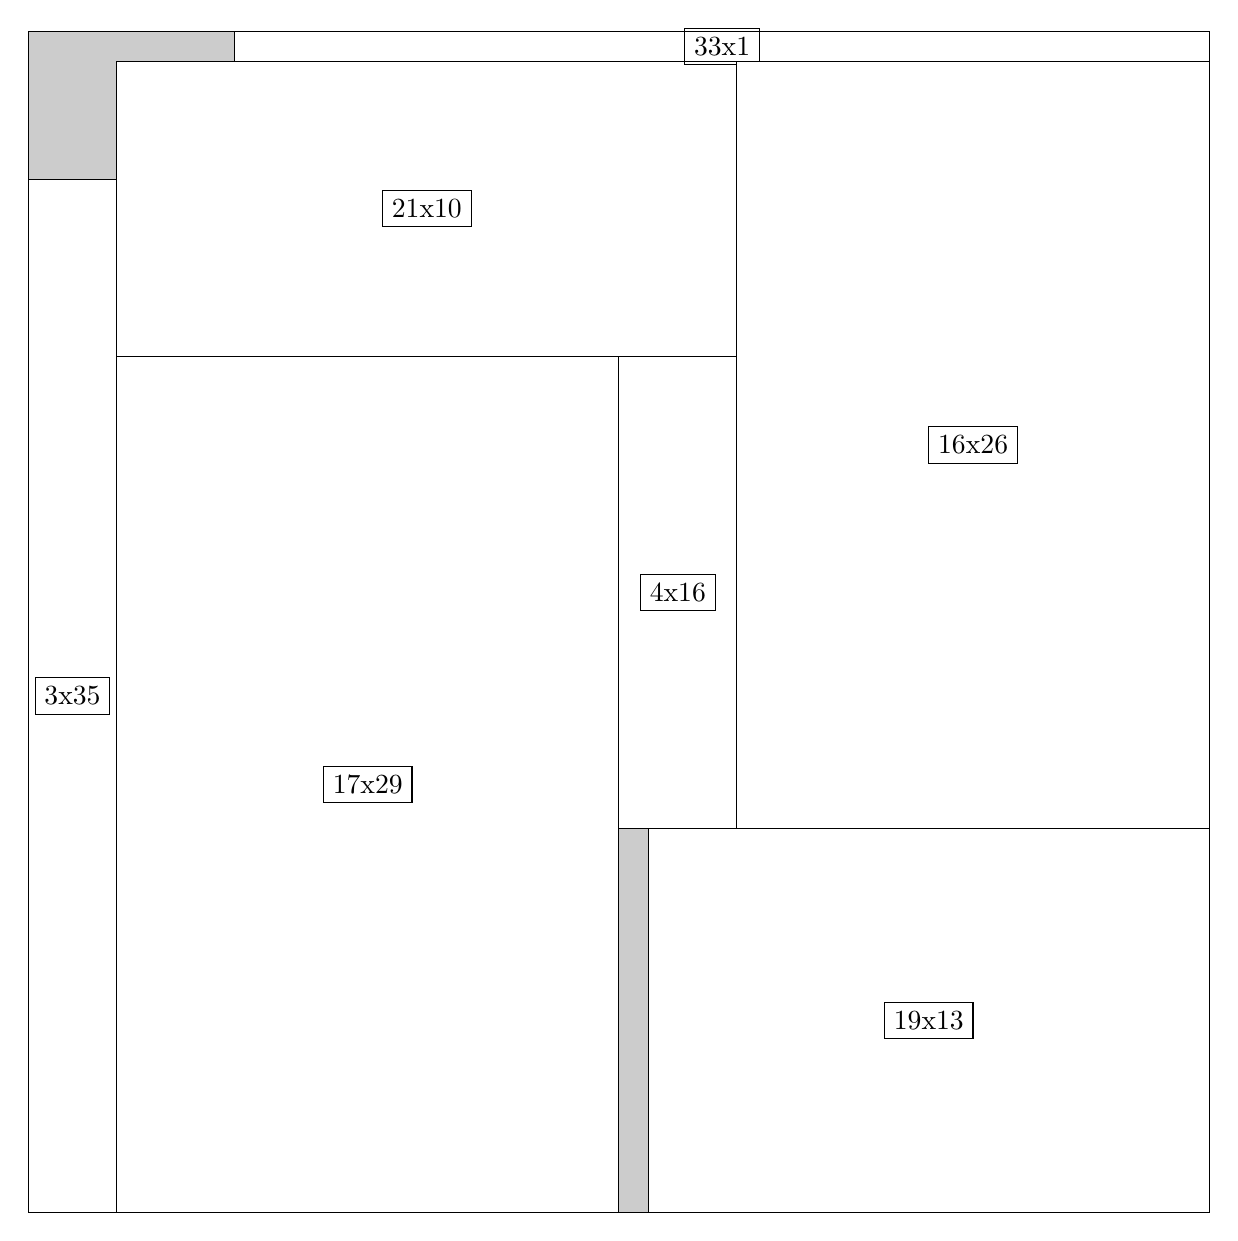
\begin{tikzpicture}[shorten >=1pt,scale=1.0,every node/.style={scale=1.0},->]
\tikzstyle{vertex}=[circle,fill=black!25,minimum size=14pt,inner sep=0pt]
\filldraw[fill=gray!40!white, draw=black] (0,0) rectangle (15.0,15.0);
\foreach \name/\x/\y/\w/\h in {3x35/0.0/0.0/1.125/13.125,17x29/1.125/0.0/6.375/10.875,21x10/1.125/10.875/7.875/3.75,33x1/2.625/14.625/12.375/0.375,4x16/7.5/4.875/1.5/6.0,19x13/7.875/0.0/7.125/4.875,16x26/9.0/4.875/6.0/9.75}
\filldraw[fill=white!40!white, draw=black] (\x,\y) rectangle node[draw] (\name) {\name} ++(\w,\h);
\end{tikzpicture}


w =3 , h =35 , x =0 , y =0 , v =105
\par
w =17 , h =29 , x =3 , y =0 , v =493
\par
w =21 , h =10 , x =3 , y =29 , v =210
\par
w =33 , h =1 , x =7 , y =39 , v =33
\par
w =4 , h =16 , x =20 , y =13 , v =64
\par
w =19 , h =13 , x =21 , y =0 , v =247
\par
w =16 , h =26 , x =24 , y =13 , v =416
\par
\newpage


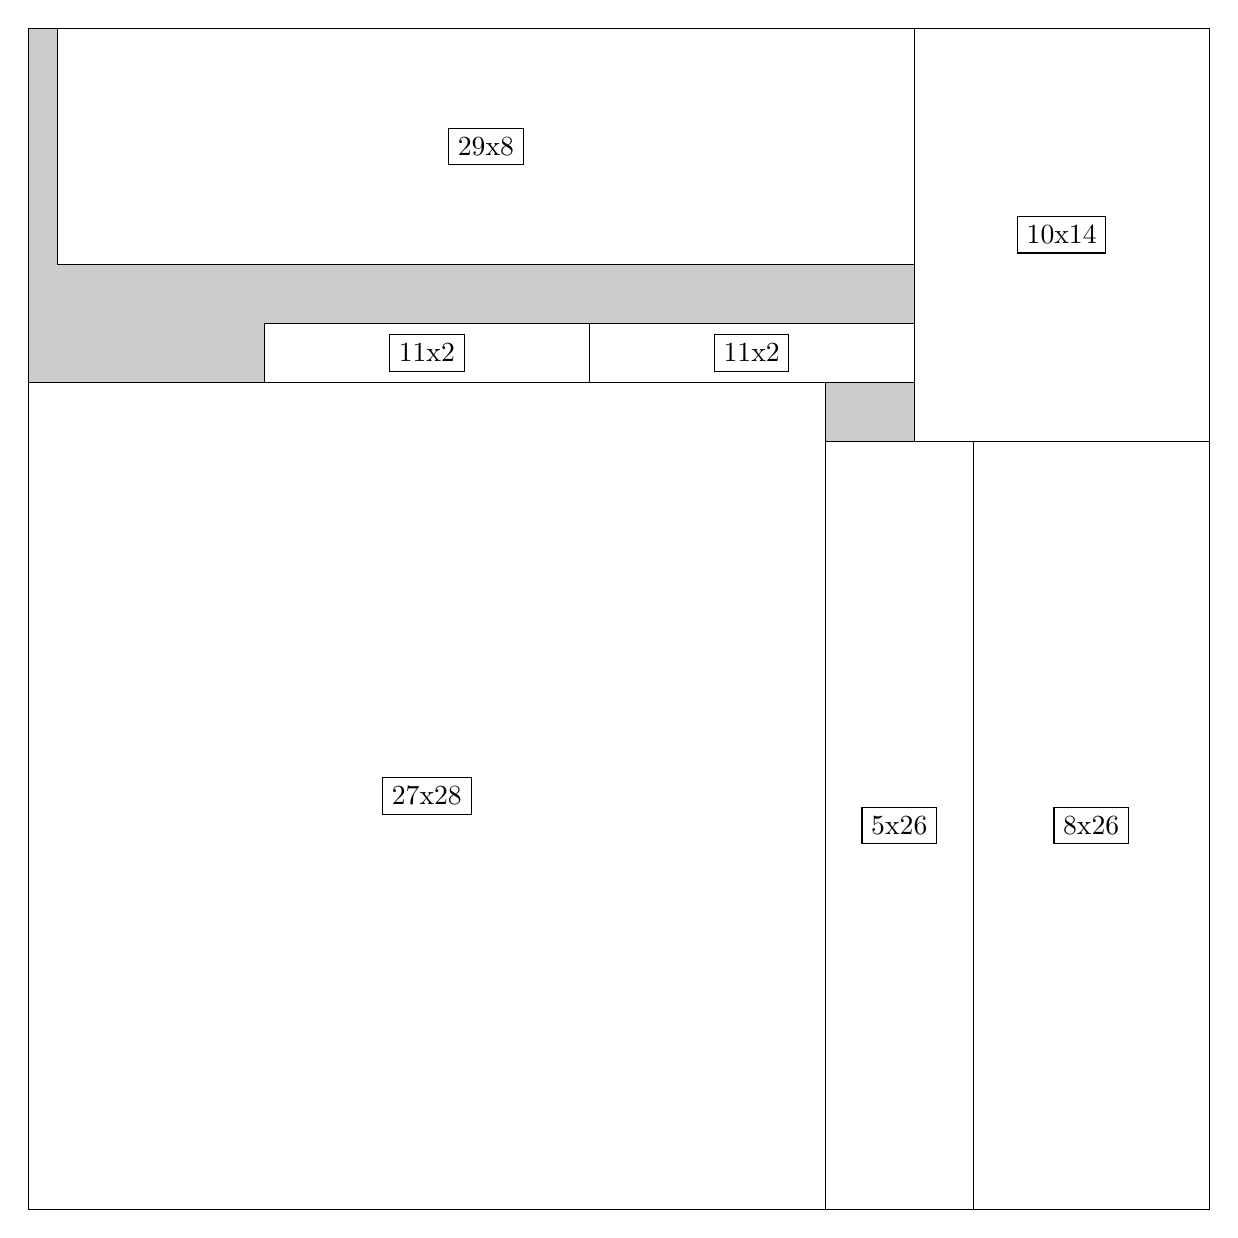
\begin{tikzpicture}[shorten >=1pt,scale=1.0,every node/.style={scale=1.0},->]
\tikzstyle{vertex}=[circle,fill=black!25,minimum size=14pt,inner sep=0pt]
\filldraw[fill=gray!40!white, draw=black] (0,0) rectangle (15.0,15.0);
\foreach \name/\x/\y/\w/\h in {27x28/0.0/0.0/10.125/10.5,8x26/12.0/0.0/3.0/9.75,5x26/10.125/0.0/1.875/9.75,10x14/11.25/9.75/3.75/5.25,11x2/7.125/10.5/4.125/0.75,11x2/3.0/10.5/4.125/0.75,29x8/0.375/12.0/10.875/3.0}
\filldraw[fill=white!40!white, draw=black] (\x,\y) rectangle node[draw] (\name) {\name} ++(\w,\h);
\end{tikzpicture}


w =27 , h =28 , x =0 , y =0 , v =756
\par
w =8 , h =26 , x =32 , y =0 , v =208
\par
w =5 , h =26 , x =27 , y =0 , v =130
\par
w =10 , h =14 , x =30 , y =26 , v =140
\par
w =11 , h =2 , x =19 , y =28 , v =22
\par
w =11 , h =2 , x =8 , y =28 , v =22
\par
w =29 , h =8 , x =1 , y =32 , v =232
\par
\newpage


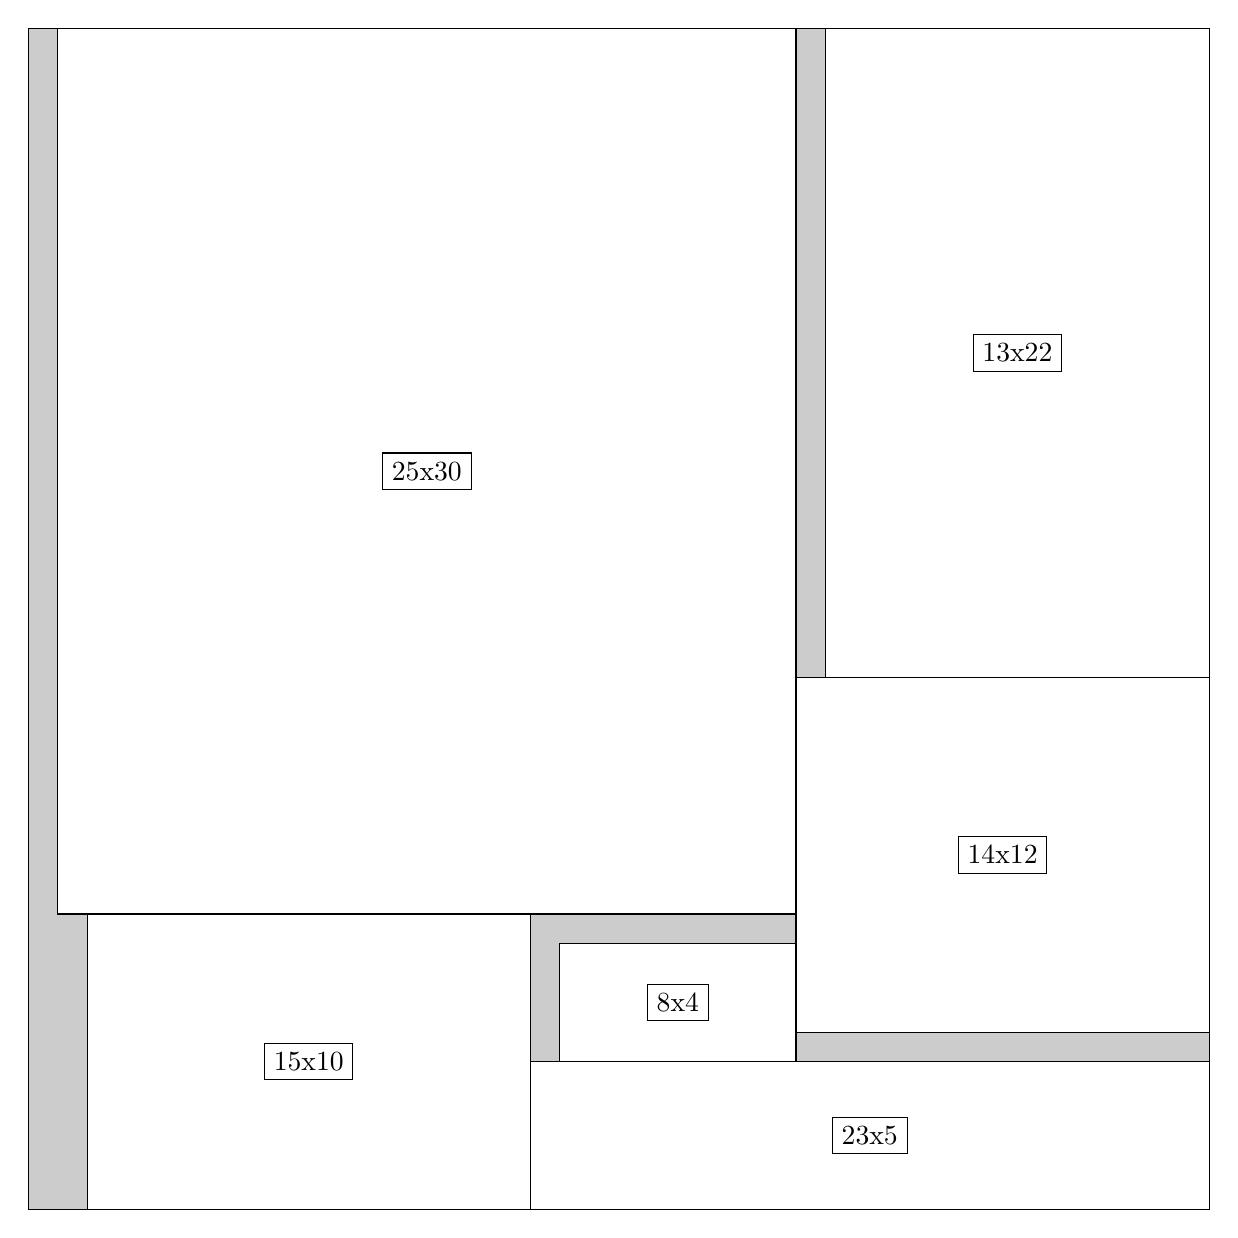
\begin{tikzpicture}[shorten >=1pt,scale=1.0,every node/.style={scale=1.0},->]
\tikzstyle{vertex}=[circle,fill=black!25,minimum size=14pt,inner sep=0pt]
\filldraw[fill=gray!40!white, draw=black] (0,0) rectangle (15.0,15.0);
\foreach \name/\x/\y/\w/\h in {23x5/6.375/0.0/8.625/1.875,15x10/0.75/0.0/5.625/3.75,8x4/6.75/1.875/3.0/1.5,14x12/9.75/2.25/5.25/4.5,25x30/0.375/3.75/9.375/11.25,13x22/10.125/6.75/4.875/8.25}
\filldraw[fill=white!40!white, draw=black] (\x,\y) rectangle node[draw] (\name) {\name} ++(\w,\h);
\end{tikzpicture}


w =23 , h =5 , x =17 , y =0 , v =115
\par
w =15 , h =10 , x =2 , y =0 , v =150
\par
w =8 , h =4 , x =18 , y =5 , v =32
\par
w =14 , h =12 , x =26 , y =6 , v =168
\par
w =25 , h =30 , x =1 , y =10 , v =750
\par
w =13 , h =22 , x =27 , y =18 , v =286
\par
\newpage


\end{document}